% \documentclass[10pt]{article} 

\usepackage{amsmath,amssymb,amsthm,amsfonts} % assumes amsmath package installed
\usepackage[linktocpage=true,colorlinks=true,linkcolor=blue,citecolor=blue,urlcolor=blue]{hyperref}
\usepackage[letterpaper,margin=0.9in]{geometry}

% \newtheorem{definition}{Definition}
% \newtheorem{assumption}{Assumption}
% \newtheorem{theorem}{Theorem}
% \newtheorem{conjecture}{Conjecture}
% \newtheorem{lemma}{Lemma}
% \newtheorem{proposition}{Proposition}
% \newtheorem{remark}{Remark}

\newcommand{\bx}{\boldsymbol{x}}
\newcommand{\be}{\boldsymbol{e}}
\newcommand{\blambda}{\boldsymbol{\lambda}}
\newcommand{\bLambda}{\boldsymbol{\Lambda}}
\newcommand{\bu}{\boldsymbol{u}}
\newcommand{\bw}{\boldsymbol{w}}
\newcommand{\by}{\boldsymbol{y}}
\newcommand{\bz}{\boldsymbol{z}}
\newcommand{\bV}{\boldsymbol{V}}
\newcommand{\bX}{\boldsymbol{X}}
\newcommand{\bY}{\boldsymbol{Y}}
\newcommand{\bZ}{\boldsymbol{Z}}
\newcommand{\bv}{\boldsymbol{v}}
\newcommand{\bxi}{\boldsymbol{\xi}}
\newcommand{\bpi}{\boldsymbol{\pi}}
\newcommand{\bphi}{\boldsymbol{\phi}}
\newcommand{\bbeta}{\boldsymbol{\eta}}
\newcommand{\bpsi}{\boldsymbol{\psi}}
\newcommand{\bzeta}{\boldsymbol{\zeta}}
\newcommand{\bmu}{\boldsymbol{\mu}}
\newcommand{\bq}{\boldsymbol{q}}
\newcommand{\bQ}{\boldsymbol{Q}}
\newcommand{\bK}{\boldsymbol{K}}
\newcommand{\bP}{\boldsymbol{P}}
\newcommand{\bS}{\boldsymbol{S}}
\newcommand{\bT}{\boldsymbol{T}}
\newcommand{\bF}{\boldsymbol{F}}
\newcommand{\bG}{\boldsymbol{G}}
\newcommand{\bd}{\boldsymbol{d}}
\newcommand{\bp}{\boldsymbol{p}}
\newcommand{\bff}{\boldsymbol{f}}
\newcommand{\bc}{\boldsymbol{c}}
\newcommand{\bg}{\boldsymbol{g}}
\newcommand{\bh}{\boldsymbol{h}}
\newcommand{\bA}{\boldsymbol{A}}
\newcommand{\bL}{\boldsymbol{L}}
\newcommand{\ba}{\boldsymbol{a}}
\newcommand{\bb}{\boldsymbol{b}}
\newcommand{\bB}{\boldsymbol{B}}
\newcommand{\bC}{\boldsymbol{C}}
\newcommand{\bE}{\boldsymbol{E}}
\newcommand{\bH}{\boldsymbol{H}}
\newcommand{\bR}{\boldsymbol{R}}
\newcommand{\bn}{\boldsymbol{n}}
\newcommand{\bm}{\boldsymbol{m}}
\newcommand{\br}{\boldsymbol{r}}
\newcommand{\bl}{\boldsymbol{l}}
\newcommand{\bI}{\boldsymbol{I}}
\newcommand{\osigma}{\overline{\sigma}}
\newcommand{\usigma}{\underline{\sigma}}
\newcommand{\oosigma}{\overline{\osigma}}
\newcommand{\uusigma}{\underline{\usigma}}
\newcommand{\olambda}{\overline{\lambda}}
\newcommand{\ulambda}{\underline{\lambda}}
\newcommand{\oolambda}{\overline{\olambda}}
\newcommand{\uulambda}{\underline{\ulambda}}
\newcommand{\bzero}{\boldsymbol{0}}
\newcommand{\dist}{\text{\normalfont dist}}
\newcommand{\st}{\mathop{\text{\normalfont s.t.}}}
\newcommand{\diag}{\mathop{\text{\normalfont diag}}}
\newcommand{\amin}{\mathop{\text{\normalfont argmin}}}
\newcommand{\ReH}{\mathop{\text{\normalfont ReH}}}
\newcommand{\bbZ}{\mathbb{Z}}
\newcommand{\cG}{\mathcal{G}}
\newcommand{\cV}{\mathcal{V}}
\newcommand{\cW}{\mathcal{W}}
\newcommand{\cA}{\mathcal{A}}
\newcommand{\cB}{\mathcal{B}}
\newcommand{\cL}{\mathcal{L}}
\newcommand{\cE}{\mathcal{E}}
\newcommand{\cD}{\mathcal{D}}
\newcommand{\cP}{\mathcal{P}}
\newcommand{\cQ}{\mathcal{Q}}
\newcommand{\cK}{\mathcal{K}}
\newcommand{\cM}{\mathcal{M}}
\newcommand{\cN}{\mathcal{N}}
\newcommand{\cI}{\mathcal{I}}
\newcommand{\cJ}{\mathcal{J}}
\newcommand{\cT}{\mathcal{T}}
\newcommand{\interior}{\mathop{\text{\normalfont interior}}}
\newcommand{\relint}{\mathop{\text{\normalfont relint}}}
\newcommand{\vertices}{\mathop{\text{\normalfont vertices}}} 
\sloppy
\usepackage{graphicx}

\usepackage{enumitem} 
\usepackage{mathtools}
\allowdisplaybreaks
\renewcommand{\theenumi}{(\alph{enumi})} 
\usepackage{parskip}

\usepackage{tikz}

\usepackage{multirow}
\usepackage{pifont}
\newcommand{\cmark}{\ding{51}}%
\newcommand{\xmark}{\ding{55}}%


\title{Accelerating Optimal Power Flow with GPUs: SIMD Abstraction of Nonlinear Programs and Condensed-Space Interior-Point Methods
}


\date{\small
  $^{1}$Mathematics and Computer Science Division, Argonne National Laboratory\\
  $^{2}$Centre Automatique et Syst\`{e}mes, Mines Paris - PSL
}
\begin{document}
\maketitle
\begin{abstract}
  This paper introduces a novel computational framework for solving
alternating current optimal power flow (ACOPF) problems using
graphics processing units (GPUs). While GPUs have demonstrated
remarkable performance in various computing domains, their application
in AC OPF has been limited due to challenges associated with porting
sparse automatic differentiation (AD) and spars e linear solver
routines to GPUs. We aim to address these issues with two key
strategies. First, we utilize a single-instruction, multiple-data
(SIMD) abstraction of nonlinear programs (NLP). This approach enables
the specification of model equations while preserving their
parallelizable structure, and in turn, facilitates the implementation
of AD routines that can exploit such structure. Second, we employ a
condensed-space interior-point method (IPM) with an inequality
relaxation strategy. This technique involves relaxing equality
constraints to inequalities and condensing the Karush-Kuhn-Tucker
system into a much smaller positive definite system. This strategy
offers the key advantage of being able to factorize the KKT matrix
without numerical pivoting, which in the past has hampered the parallelization of
the IPM algorithm. By combining these two strategies, we can perform the
majority of operations on GPUs while keeping the data residing in the
device memory only. Comprehensive numerical benchmark results showcase
the substantial computational advantage of our approach. Remarkably,
for solving large-scale AC OPF problems to a moderate accuracy, our
implementations—MadNLP.jl and SIMDiff.jl—running on NVIDIA GPUs
achieve an order of magnitude speedup compared to state-of-the-art
tools running on contemporary CPUs.
\end{abstract}

\begin{IEEEkeywords}
  nonlinear programming, automatic differentiation, GPU computing, optimal power flow
\end{IEEEkeywords}
\section{Introduction}

The adoption of GPUs in the mathematical programming community has remained
limited. Notably, nonlinear programming (NLP) remains dependent on
algorithms developed in the 1990s offering limited room for parallelism.
One of the primary challenges arises from the
automatic differentiation (AD) of sparse model equations and the
parallel factorization of indefinite sparse matrices, which are
commonly encountered within constrained numerical optimization tasks
\cite{anitescu2021targeting}. While GPU computation can trivially
accelerate several parts of the optimization process --- especially
various internal computations within the optimization solver --- the
sluggish data transfer between host and device memory hampers the
ad-hoc implementation of GPU accelerations (Fig. \ref{fig:memory}). To
fully leverage the potential offered by modern GPU hardware, it
becomes imperative to have a comprehensive computational framework for
optimization on GPUs. That is, we need an AD/algebraic
modeling framework, sparse linear solvers, and NLP solvers that can
operate entirely on the GPU. Specifically, for the best performance,
both the problem data and the solver's intermediate computational data
must be exclusively resident within the device memory, with the
majority of operations executed on the GPU.

\begin{figure}[t]
  \centering
  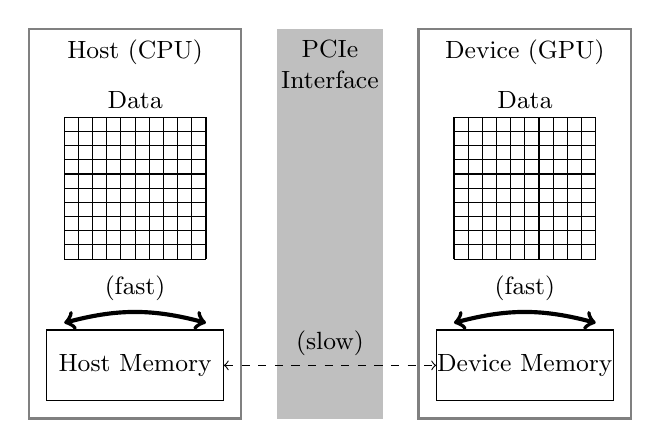
\begin{tikzpicture}[remember picture, scale=.9, font=\small]

    \fill[lightgray] (3.25,-.75) rectangle (4.75,4.75) node[black,midway,align=center,yshift=57.5] {PCIe\\Interface};
    \draw[gray,thick] (-.25,-.75) rectangle (2.75,4.75) node[black,midway,align=center,yshift=62] {Host (CPU)};
    \draw[gray,thick] (5.25,-.75) rectangle (8.25,4.75) node[black,midway,align=center,yshift=62] {Device (GPU)};

    \node[align=center] at (1.25, 3.75) {Data};
    \node[align=center] at (6.75, 3.75) {Data};

    % Host Memory
    \draw (0,-.5) rectangle (2.5,.5) node[midway] {Host Memory};

    % Device Memory
    \draw (5.5,-.5) rectangle (8,.5) node[midway] {Device Memory};


    % Arrow with Dashed Line
    \draw[<->, dashed] (2.5, 0) -- (5.5, 0) node[midway, above, align=center] {(slow)};
    \draw[<->, line width=1.5] (.25, .6) to [in=165, out =15] node[midway, above, align=center] {(fast)}(2.25, .6) ;
    \draw[<->, line width=1.5] (5.75, .6) to [in=165, out =15] node[midway, above, align=center] {(fast)}(7.75, .6) ;

    \def\rows{10}
    \def\cols{10}
    \def\elementwidth{2}
    \foreach \xshift/\yshift in {.25/1.5, 5.75/1.5} {

      % Draw Grid
      \foreach \i in {0,...,\rows} {
        \draw (\xshift, \yshift+\i*\elementwidth/\rows) -- (\xshift+\elementwidth, \yshift+\i*\elementwidth/\rows);
      }
      \foreach \i in {0,...,\cols} {
        \draw (\xshift+\i*\elementwidth/\cols, \yshift) -- (\xshift+\i*\elementwidth/\cols, \yshift+\elementwidth);
      }
    }
  \end{tikzpicture}
  \caption{A schematic description of host (CPU) and device (GPU) memory.}\label{fig:memory}
\end{figure}

This paper presents our approach to implement a comprehensive
computational framework for solving large-scale AC OPF problems on
NVIDIA GPUs, along with the associated software implementations:
SIMDiff.jl \cite{simdiff}, an algebraic modeling/AD tool, and MadNLP.jl \cite{madnlp}, an
NLP solver. Our approach incorporates two novel strategies: (i) a
single-instruction, multiple-data (SIMD) abstraction of nonlinear
programs (NLPs), enabling streamlined parallel AD on GPUs, and (ii) a
condensed-space interior-point method (IPM) with an inequality
relaxation strategy, which facilitates the use of highly efficient
{\it refactorization} routines for sparse matrix factorization with
fixed pivot sequences.


While derivative evaluation can be generally cheaper than linear
algebra operations, our numerical results on AC OPF problems show that
AD often constitutes more than half of the total solver time when
using off-the-shelf AD implementations like
JuMP.jl~\cite{dunning2017jump} or
AMPL~\cite{fourer1990modeling}. Instead, our method leverages a
specialized AD implementation based on the SIMD abstraction of
NLPs. This abstraction allows to preserve the parallelizable structure
within the model equations, facilitating efficient derivative
evaluations on the GPU. The AC power flow model is particularly
well-suited for this abstraction as it involves repetitive expressions
for each component type (e.g., buses, lines, generators), and the
number of computational patterns does not increase with the network's
size. Numerical results reported in this paper demonstrate that our
proposed strategies can achieve over 20 times speedup by running on
GPU. In comparison to general AD implementations on CPUs (such as AMPL
and JuMP.jl), our GPU-based differentiation method can be
approximately 500 times faster.

Linear algebra operations, especially sparse indefinite matrix
factorization, are typically the bottleneck in NLP solution methods.
Parallelizing this operation has been considered to be challenging,
primarily due to the need for numerical pivoting, which is sequential
in nature. However, when the matrix can be factorized without
numerical pivoting, a significant part of the operation can be
parallelized, and the numerical factorization can be efficiently
performed on GPUs. We develop a condensed-space IPM strategy that
allows the use of sparse matrix factorization routines without
numerical pivoting. This strategy relaxes equality constraints by
permitting small violations, which enables expressing the
Karush-Kuhn-Tucker (KKT) system entirely in the primal space through
the condensation procedure. Although this strategy is not new
\cite{nocedal2006numerical}, it has traditionally been considered less
efficient than the standard full-space method due to increased nonzero
entries in the KKT system. However, when implemented on GPUs, it
offers the key advantage of ensuring positive definiteness in the
condensed KKT system. This, in turn, allows for the utilization
of linear solvers with a fixed numerical pivot sequence (known as
refactorization), an efficient implementation of which is available in the CUDA library.
Although this method is susceptible to numerical stability issues due to
increased condition number in the KKT system, our results demonstrate
that the solver is robust enough to solve problems with a relative
accuracy of $\epsilon_{\text{mach}}^{1/4}\approx 10^{-4}$.

We present numerical benchmark results to showcase the efficiency of
our method, utilizing our two packages: MadNLP.jl and
SIMDiff.jl. The solution of the KKT system is performed using the
external {\tt cuSOLVER} library. To assess the performance of our method, we
compare it against standard CPU approaches using the data available in
pglib-opf \cite{babaeinejadsarookolaee2019power}.  Our benchmark results
demonstrate that our proposed computational framework has significant
potential for accelerating the solution of AC OPF problems, especially
when a moderate accuracy (e.g., $10^{-4}$) is sufficient.
Notably, when running on NVIDIA GPUs, our method achieves a
4x speedup compared to our solver running on CPU for
the largest instance. Moreover for the same instance, our approach
surpasses the performance of existing tools (such as Ipopt interfaced
with JuMP.jl) by an order of magnitude. This finding underscores the
importance of harnessing the power of GPUs for tackling
the computational challenges in power systems.

\paragraph*{Contributions}
We present, for the first time, a nonlinear optimization framework
that can run entirely on GPU, with all the performance-critical data
arrays residing exclusively on GPUs. Additionally, we introduce the
concept of SIMD abstraction for NLP problems, which results in an
efficient implementation of GPU-accelerated parallel AD. Furthermore,
we propose the condensed IPM with inequality relaxation strategy for
the first time, enabling the treatment of the KKT systems of NLPs
without numerical pivoting, thus allowing the solution of sparse,
large-scale NLPs (with a prominentexample being AC OPFs) on GPUs.

\paragraph*{Related Work}
Several recent works have explored the use of GPUs for large-scale
nonlinear optimization problems. Cao et al. \cite{cao2016augmented}
proposed an augmented Lagrangian interior-point approach that employs
augmented Lagrangian outer iteration and the treatment of linear
systems using a preconditioned conjugate gradient method. Prior to the
introduction of the sparse condensed-space IPM with an inequality relaxation
strategy, the authors have investigated the use of reduction
strategies (state variable elimination) to treat KKT systems in a
dense form on the GPU
\cite{pacaud2023parallel,pacaud2022feasible,pacaud2023accelerating}.
In parallel, approaches based on Lagrangian decomposition and
batched with batched TRON solver \cite{lin1999newton}
has been investigated \cite{kim2022accelerated,kim2021leveraging}.
An NLP solver for high-performance computers (HPC) with GPU
accelerators called HiOP has been under development
\cite{hiop_techrep}, with a similar scope as our solver MadNLP.jl.
 Another recent development is the hybrid (direct-iterative) KKT
system solver specifically designed for GPUs \cite{regev2023hykkt}.
The implementation of derivative evaluations with the exploitation of
repeated structures within model equations has, to the best of our
knowledge, been first introduced in Gravity \cite{Gravity}. This was
achieved through the introduction of so-called template constraints,
and multi-threaded derivate evaluation has been implemented therein.
However, it is important to note that their differentiation approach
is based on symbolic differentiation.
The idea of condensed-space IPM (without inequlaity relaxation
strategy) is not new, but they have been used primarily in more
specific contexts, where the increased nonzero entries in the KKT system
is less of a concern, such as in the dense form model predictive control
problems \cite{jerez2012sparse,cole2023exploiting}.


\paragraph*{Organization}
The paper is organized as follows. In the remainder of the current
section, we introduce the mathematical notation. In Section
\ref{sec:prelim}, we provide general preliminary knowledge on
numerical optimization, automatic differentiation, and GPU computing.
In Section \ref{sec:simd}, we present the SIMD abstraction of NLPs and
their advantages in terms of implementing parallel AD. Section
\ref{sec:ipm} presents the optimization algorithm under study, the
condensed-space IPM with an inequality relaxation strategy. Section
\ref{sec:num} presents the numerical results, comparing our approach
with other state-of-the-art solution methods on the CPUs. Finally,
conclusions and future outlooks are given in Section \ref{sec:conc}.

\paragraph*{Notation}
We denote the set of real numbers and the set of integers by
$\mathbb{R}$ and $\mathbb{I}$. We let $[M]:=\{1,2,\cdots,M\}$. We let
$[v_i]_{i\in[M]}:=[v_1;v_2;\cdots,v_M]$.  A vector of ones with an
appropriate size is denoted by $\boldsymbol{1}$. An identity matrix
with an appropriate size is denoted by $I$. For matrices $A$ and $B$,
$A\succ(\succeq) B$ indicates that $A-B$ is positive (semi)-definite
while $A>(\geq) B$ denotes a component-wise inequality. We use the
convention $X:=\diag(x)$ for any symbol $x$.

\section{Preliminaries}\label{sec:prelim}
This section covers three essential background topics: numerical
optimization, AD, and GPU computing.

\subsection{Numerical Optimization}\label{sec:numopt}
We consider NLPs of the following form:
\begin{equation}\label{eqn:cpt}
    \min_{x^\flat \leq x \leq x^\sharp}\;  f(x) \quad \st\;
     g(x) =0 \, .
\end{equation}
Numerous solution algorithms have been developed in the NLP
literature to solve \eqref{eqn:cpt}. In terms of strategies to deal with inequality
constraints, the NLP solution algorithms can be broadly classified
into active-set methods and interior-point methods (IPMs) \cite{nocedal2006numerical}.
Active-set methods aim to find the set of active constraints associated
with the optimal solution in a combinatorial manner, while IPMs
replace inequality constraints with smooth barrier functions.
IPMs are known to be
more scalable for problems with a large number of constraints and
suitable for parallelization, thanks to the fixed sparsity pattern of
the KKT matrix. Given these advantages, we have chosen IPMs as the
backbone algorithm for developing our optimization methods on GPUs.

In terms of practical computations, three key components play
vital roles: derivative evaluations (often provided by the AD
capabilities of the algebraic modeling languages), linear algebra
operations, and various internal computations within the
solver. Notably, most of the computational efforts are delegated to
the external linear solver and AD library, while the optimization solver
orchestrates the operation of these tools to drive the solution
iterate towards the stationary point of the optimization problem.

Since the successful implementation of the open-source IPM solver
Ipopt, many subsequent implementations of NLP solvers
\cite{chiang2014structured,rodriguez2023scalable,shin2021graph} have
based their implementation on Ipopt
\cite{wachter2006implementation}. We also use Ipopt as our main
reference for the IPM implementation. Below, we outline the overall
computational procedure employed within the NLP solution frameworks:

1) Given the current primal-dual iterate $(x^{(\ell)},y^{(\ell)},
z^{\flat(\ell)},z^{\sharp(\ell)})$, the AD package evaluates the first-
and second-order derivatives:
\begin{align*}
  \nabla_x f(x^{(\ell)}),\quad
  \nabla_x g(x^{(\ell)}),\quad
  \nabla^2_{xx} \mathcal{L}(x^{(\ell)},y^{(\ell)},z^{\flat(\ell)},z^{\sharp(\ell)}),
\end{align*}
where
\begin{align*}
  \mathcal{L}(x,y,z^{\flat},z^{\sharp}):=f(x) - y^\top
  g(x) - z^\flat (x-x^\flat) - z^\sharp (x^\sharp-x).
\end{align*}

2) The following sparse indefinite system (known as the KKT system) is
solved using sparse indefinite factorization (typically, via sparse
LBL$^\top$ factorization) and triangular solve routines.
\begin{align}\label{eqn:kkt-indefinite}
  &\begin{bmatrix}
    W^{(\ell)}  + \Sigma^{(\ell)} + \delta^{(\ell)}_w I& A^{(\ell)\top}\\
    A^{(\ell)} & -\delta_c^{(\ell)} I\\
  \end{bmatrix}
  \begin{bmatrix}
    \Delta x\\
    \Delta y\\
  \end{bmatrix}=
  \begin{bmatrix}
    r_x^{(\ell)}\\
    r_y^{(\ell)}\\
  \end{bmatrix},
\end{align}
where
\begin{align*}
  W^{(\ell)}
  &:=\nabla^{2}_{xx}\mathcal{L}(x^{(\ell)},y^{(\ell)},z^{\flat(\ell)},z^{\sharp(\ell)}),
  &&A^{(\ell)}:= \nabla_xg(x^{(\ell)})\\
  \Sigma^{(\ell)}&:= (X^{(\ell)})^{-1}Z^{(\ell)}\\
  r_x^{(\ell)}
  &:=\nabla_x f(x^{(\ell)}) - \mu (X^{(\ell)})^{-1} \boldsymbol{1},
  &&r_y^{(\ell)}:=g(x^{(\ell)}),
\end{align*}
and $\delta^{(\ell)}_w, \delta^{(\ell)}_c>0$ are the regularization parameters
determined based on the inertia correction procedure.

3) The optimization solver employs a filter line search procedure to
determine the step size~\cite{wachter2006implementation}. The primal-dual iterate is updated by
applying the determined step size and direction. This process is
repeated until satisfaction of the convergence criteria (typically based on the residual
to the first-order optimality conditions).

\subsection{Automatic Differentiation (AD)}
Numerical differentiation of computer programs can be achieved through
three different methods: (i) finite difference method, (ii) symbolic
differentiation, and (iii) AD. The finite difference method suffers
from numerical rounding errors, and its computational complexity grows
unfavorably with respect to the number of function arguments, making
it less preferable unless no other alternatives are
available. Symbolic differentiation uses computer algebra systems to
obtain symbolic expressions of first or higher-order
derivatives. While this method can differentiate functions up to high
numerical precision, it suffers from "expression swelling" effect and
struggles to compute the derivatives of long nested expressions in a
computationally efficient way.

In contrast, AD differentiates computer
programs directly by inspecting the computation graph and applying chain rules,
to evaluate derivatives efficiently and accurately.
This approach has become the dominant paradigm for derivative computation within the
scientific computing domain, including NLP and
machine learning. For large-scale optimization problems, such as AC
OPFs, AD tools are often implemented as part of domain-specific
modeling languages. Examples of such modeling languages include JuMP,
CasADi, and AMPL (optimization) and Tensorflow, Torch and, Flux
(machine learning).

There are two alternative ways of propagating derivatives through the
recursive application of chain rules: (i) forward-mode and (ii)
reverse-mode, which operate in opposite directions (respectively, from leaves to
root and from root to leaves). Reverse-mode automatic
differentiation, also known as the adjoint method, has proven to be
particularly effective for dealing with function expressions in
large-scale optimization problems.

The Julia Language, our language of choice, offers convenient and
efficient ways to implement automatic differentiation. Through the use
of the multiple dispatch paradigm~\cite{bezanson2017julia} \textit{any
Julia function}---including commonly used operations like addition,
multiplication, trigonometric and exponential functions (among
others)---can be easily overloaded. Multiple dispatch allows functions
to be dynamically dispatched based on the run-time type, a crucial
feature for implementing differentiable programming. Several AD
implementations have been developed in Julia Language, such as
ReverseDiff.jl, ForwardDiff.jl, Zygote.jl, and JuMP.jl. While these
tools are general and useful for various applications, they are not
optimized for evaluating derivatives of AC OPF problems, as they are
not designed to exploit the parallelizable structures in the model,
while preserving the desired sparsity.


\subsection{GPU Computing}\label{sec:gpu}
With the increasing prevalence of GPU in various scientific computing
domains, there has been growing interest in leveraging these emerging
architectures to efficiently solve large-scale NLPs, like AC OPF problems.
However, adapting a NLP solution algorithms,
such as IPM, to GPUs presents challenges due to the fundamental
differences between GPU and CPU programming paradigms. While CPUs
execute a sequence of instructions on a single input (single
instruction, single data, or SISD, in Flynn's taxonomy), GPUs run the
same instruction simultaneously on hundreds of threads using the SIMD
paradigm (see Fig. \ref{fig:simd}). The SIMD parallelism works well
for algorithms that can be decomposed into simple instructions running
entirely in parallel, but not all algorithms fit this
paradigm. For example, branching in the control flow can hinder
lockstep execution across multiple threads, and in turn, prevent
efficient implementations on GPUs. On the contrary, when the
algorithm's structure allows for efficient parallelization, the SIMD
parallelism in GPUs can offer orders of magnitudes speedup.

We highlight that the following, arguably common, computational
patterns are particularly effective when implemented on GPUs:
\begin{align}
  y&\leftarrow \left[\phi(x; q_j)\right]_{j\in [J]}\tag{Pattern 1}\label{eqn:pattern-1}\\
  o&\leftarrow  \mathop{\rm{Op}}_{i\in [I]} \psi(x;p_i) \tag{Pattern 2}\label{eqn:pattern-2}\\
  x&\leftarrow  \chi_{s_1}\circ\cdots\circ \chi_{s_K}(x) \tag{Pattern 3}\label{eqn:pattern-3}
\end{align}
Here, $\psi:\mathbb{R}^{n_x}\times \mathbb{R}^{n_{p}}\rightarrow
\mathbb{R}$ , $\phi:\mathbb{R}^{n_x}\times
\mathbb{R}^{n_{q}}\rightarrow \mathbb{R}$, and
$\chi:\mathbb{R}^{n_x}\times \mathbb{R}^{n_{s}}\rightarrow
\mathbb{R}^{n_x}$ are simple instructions that require only a small number
of operations; $\mathop{\rm{Op}}$ is a monoid operator on
$\mathbb{R}\cup\{+\infty,-\infty\}$, such as addition, multiplication,
maximum, and minimum. In \ref{eqn:pattern-3}, we denote $\chi_{s_k}(x):=\chi(x,s_k)$ and
assume that $\circ$ is commutative for $\{\chi_{s_k}(\cdot)\}_{\forall
s_k}$. \ref{eqn:pattern-1} is typically most effective on GPUs, where
each thread employed can operate independently without needing to
simultaneously manipulate the same device memory location. While
\ref{eqn:pattern-2} and \ref{eqn:pattern-3} are less effective,
they still can be significantly
faster than operations on CPUs, as substantial part of the operation
can still be parallelized by the use of buffers. In simple cases, the
implementation of these operations can be performed with the standard
{\tt map} and {\tt mapreduce} programming models. However, in more
complex cases, especially for \ref{eqn:pattern-3}, the implementation
may require pre-inspection of memory write-access patterns and the use
of custom kernels.

Many of the operations required in AD of sparse physical models, as
well as the application of optimization algorithms, are based on the
computational patterns mentioned above. For example, an AC OPF model
can be implemented with 15 different computational patterns (see
Section~\ref{sec:simd:ad}), all of which fall within the
aforementioned categories. Furthermore, the computation within
optimization solvers, such as forming the left-hand-side for the KKT
systems, computing the $\|\cdot\|_\infty$ norm of the constraint
violation, and assembling the condensed KKT system, can be carried out
by using these computational patterns as well. The only exception is
the factorization of the sparse KKT matrix, which requires more
sophisticated implementations.

Implementing kernel functions for the above computational patterns in
the Julia Language is straightforward, as Julia provides excellent
high-level interfaces for array and kernel programming for GPU
arrays. The code can even be device-agnostic, thanks to the portable
programming capabilities brought by KernelAbstractions.jl. All
of the AD and optimization capabilities in our
tools, MadNLP.jl and SIMDiff.jl, are implemented in the Julia Language,
by leveraging its kernel and array programming capabilities.

\begin{figure}[t]
  \centering
  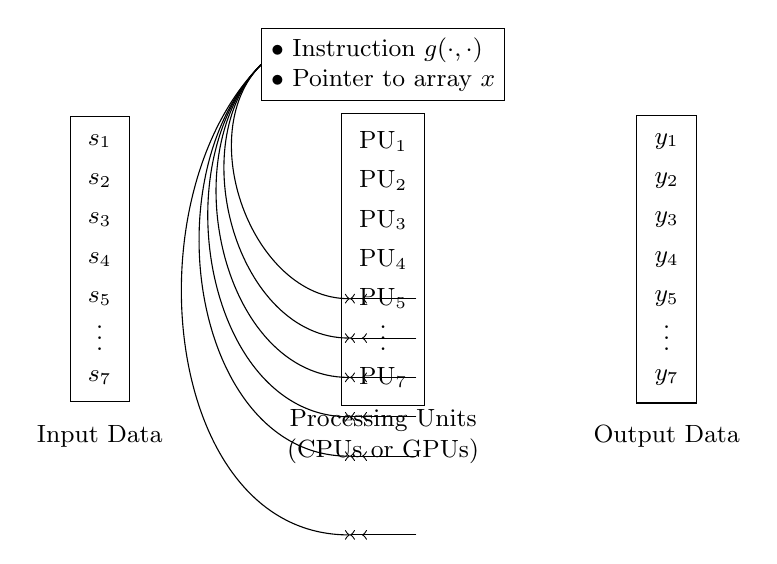
\begin{tikzpicture}[remember picture, scale=.9, font=\small]
    \node[draw,align=left] (I) at (0,2.75) {
      $\bullet$ Instruction $g(\cdot,\cdot)$\\
      $\bullet$ Pointer to array $x$
    };
    \node[draw] at (-4,0) {
      \tikz{
        \foreach\x in {1,2,3,4,5,7}{
          \node (A\x) at (0,-\x/2) {$s_{\x}$};
        }
        \node at (0,-2.9) {$\vdots$};
      }
    };
    \node[draw] at (0,0) {
      \tikz{
        \foreach\x in {1,2,3,4,5,7}{
          \node (B\x) at (0,-\x/2) {$\text{PU}_{\x}$};
        }
        \node at (0,-2.9) {$\vdots$};
      }
    };
    \node[draw] at (4,0) {
      \tikz{
        \foreach\x in {1,2,3,4,5,7}{
          \node (C\x) at (0,-\x/2) {$y_{\x}$};
        }
        \node at (0,-2.9) {$\vdots$};
      }
    };
    \foreach\x in {1,2,3,4,5,7}{
      \draw[->] (A\x.east) -- (B\x.west);
      \draw[->] (B\x.east) -- (C\x.west);
      \draw[->] (I.west) to [out=-135,in=180] (B\x.west);
    }
    \node at (-4,-2.5) {Input Data};
    \node[align=center] at (0,-2.5) {Processing Units\\(CPUs or GPUs)};
    \node at (4,-2.5) {Output Data};
  \end{tikzpicture}
  \label{fig:simd}
  \caption{A schematic description of SIMD parallelism}
\end{figure}

\section{SIMD Abstraction of NLPs}\label{sec:simd}

This section describes our implementation of SIMD abstraction and
sparse AD of the model equations. The abstraction and AD are
implemented as part of our algebraic modeling language SIMDiff.jl.

\subsection{Abstraction}
The SIMD abstraction under consideration is as follows:
\begin{align}\label{eqn:prob}
  \min_{x^\flat\leq x \leq x^\sharp}
  & \sum_{l\in[L]}\sum_{i\in [I_l]} f^{(l)}(x; p^{(l)}_i)\\\nonumber
  \st\; &\forall m\in[M]:\\\nonumber
  &\begin{aligned}[t]
    \left[g^{(m)}(x; q_j)\right]_{j\in [J_m]} +\sum_{n\in [N_m]}\sum_{k\in [K_n]}h^{(n)}(x; s^{(n)}_{k}) =0,
  \end{aligned}
  \end{align}
where $f^{(\ell)}(\cdot,\cdot)$, $g^{(m)}(\cdot,\cdot)$, and
$h^{(n)}(\cdot,\cdot)$ are twice differentiable functions with respect
to the first argument, whereas $\{\{p^{(k)}_i\}_{i\in [N_k]}\}_{k\in[K]}$,
$\{\{q^{(k)}_{i}\}_{i\in [M_l]}\}_{m\in[M]}$, and
$\{\{\{s^{(n)}_{k}\}_{k\in[K_n]}\}_{n\in[N_m]}\}_{m\in[M]}$ are
problem data, which can either be discrete or continuous.  We assume
that our functions $f^{(l)}(\cdot,\cdot)$, $g^{(m)}(\cdot,\cdot)$, and
$h^{(n)}(\cdot,\cdot)$ can be expressed with computational
graphs of moderate length. One can observe that the problem in
\eqref{eqn:prob} is expressed by the computational patterns in Section
\ref{sec:gpu}. In particular, the objective function falls within \ref{eqn:pattern-2},
the first term in the constraint falls within \ref{eqn:pattern-1}, and the second term in the constraint falls within \ref{eqn:pattern-3}.
Accordingly, the evaluation and differentiation of the
model equations in \eqref{eqn:prob} is amenable to SIMD parallelism.

To implement the SIMD abstraction in the modeling environment, the
algebraic modeling interface in SIMDiff.jl enforces the users to
specify the model equations in an {\tt Iterable} data type in
Julia Language. This composite data type consists of an instruction (a Julia
function) and data (a host or device array) over which the instruction
is executed. This naturally facilitates maintaining the NLP model
information in the form of SIMD abstraction in \eqref{eqn:prob}, and
facilitates the model evaluation and differentiation on GPU
accelerators.

\subsection{Parallel AD}
\label{sec:simd:ad}
Many physics-based models, such as AC OPF, have a highly repetitive
structure. One of the manifestations of it is that the mathematical
statement of the model is concise, even if the practical model may contain
millions of variables and constraints. This is possible due to the use of
repetition over a certain index and data sets. For example,
it suffices to use 15 computational patterns to fully specify the
AC OPF model. These patterns arise from (1) generation cost, (2) reference
bus voltage angle constraint, (3-6) active and reactive power flow (from and to),
(7) voltage angle difference constraint, (8-9) apparent
power flow limits (from and to), (10-11) power balance equations,
(12-13) generators' contributions to the power balance equations, and
(14-15) in/out flows contributions to the power balance
equations. However, such repetitive structure is not well exploited in
the standard NLP modeling paradigms. In fact, without the SIMD
abstraction, it is difficult for the AD package to detect the
parallelizable structure within the model, as it will require the full
inspection of the computational graph over all expressions.  By
preserving the repetitive structures in the model, the repetitive
structure can be directly available in AD implementation.

Using the multiple dispatch feature of Julia, SIMDiff.jl generates
highly efficient derivative computation code, specifically compiled
for each computational pattern in the model. These derivative
evaluation code can be run over the data in various GPU array formats,
implemented via array and kernel programming in Julia Language. In
turn, SIMDiff.jl has the capability to efficiently evaluate first and
second order derivatives using GPU accelerators.

\subsection{Sparsity Analysis}
The sparsity analysis is needed for determining the sparsity pattern
of the evaluated derivatives. In the case of large-scale sparse
problems, the initial sparsity analysis of nonlinear expressions can
be expensive, as the sparsity should be analyzed for potentially
millions of objective and constraints terms. However, oftentimes
these analyses are applied for the same computational patterns, and
the time and memory spent for sparsity analysis can be significantly
reduced if the repetitive structures are exploited.

SIMDiff.jl exploits the SIMD abstraction of the model equations to
save the computational cost spent for sparsity analysis.  This is
accomplished by applying sparsity analysis for the instruction for
each computational pattern and expand the obtained sparsity pattern
over the data over which the instruction is executed. Specifically,
the sparsity analysis code exploits Julia's multiple dispatch feature
to obtain a parameterized sparsity pattern for each instruction, and the
obtained parameterized sparsity pattern is materialized once the data
array is given. This process drastically saves in computational cost
for the sparsity analysis.

\section{Condensed-Space IPMs with an Inequality Relaxation Strategy}\label{sec:ipm}
We present the condensed-space IPM within the
context of the general NLP formulation in \eqref{eqn:cpt}. Our method
has two key differences from standard IPM
implementations: (i) the use of inequality relaxation and (ii) the
condensed treatment of the KKT system.

\subsection{Inequality Relaxation}

At the beginning of the algorithm, we apply inequality relaxation to replace the equality constraints in \eqref{eqn:cpt} with inequalities by introducing slack variables $s\in\mathbb{R}^{m}$:
\begin{align}\label{eqn:relax}
  g(x)- s = 0,\quad s^{\flat}\leq s\leq  s^\sharp,
\end{align}
where $s^\flat,s^\sharp\in\mathbb{R}^{m}$ are lower and upper bounds chosen to be close to zero.
This relaxed problem can be stated as follows:
\begin{equation}\label{eqn:relaxed}
    \min_{\big[\substack{x^\flat\\s^\flat}\big]\leq \big[\substack{x\\s}\big] \leq \big[\substack{x^\sharp\\s^\sharp}\big]}\;
      f(x)\quad \st\;  g(x) - s = 0 \, .
\end{equation}
In our implementation, we set $s^{\flat},s^\sharp$ as
$-\epsilon_{\text{tol}}\boldsymbol{1}$ and $+\epsilon_{\text{tol}}\boldsymbol{1}$, respectively,
where $\epsilon_{\text{tol}}>0$ is a user-specified relative tolerance
of the IPM. This type of relaxation is
commonly used in practical IPM implementations; for example, in Ipopt,
the solver relaxes the bounds and inequality constraints by
$O(\epsilon_{\text{tol}})$ to prevent an empty interior of the
feasible set (see \cite[Section 3.5]{wachter2006implementation}).
For condensed-space IPM, we cannot maintain the same level of precision
due to the increased condition number of the KKT system.
We have found that setting $\epsilon_{\text{tol}}$ to be
$\epsilon_{\text{mach}}^{1/4}\approx 10^{-4}$ ensures numerical
stability while achieving satisfactory convergence behavior. Thus, our
solver sets the $\epsilon_\text{tol}$ to $10^{-4}$ by default when using condensed
IPM.

\subsection{Barrier Subproblem}

The IPM replaces the equality and inequality-constrained problem in \eqref{eqn:relax} with an equality-constrained  barrier subproblem:
\begin{subequations}\label{eqn:barrier}
  \begin{align}
    \min_{x, s}\;
    &
      \begin{aligned}[t]
        &f(x) - \mu\boldsymbol{1}^\top \log (x- x^\flat) -\mu\boldsymbol{1}^\top \log (x^\sharp -x)\\
        &- \mu\boldsymbol{1}^\top \log (s- s^\flat) -\mu\boldsymbol{1}^\top \log (s^\sharp -s)
      \end{aligned}
          \label{eqn:barrier-obj}\\
    \st\;
    &g(x) - s = 0. \label{eqn:barrier-con}
  \end{align}
\end{subequations}
Here, $\mu>0$ is the barrier parameter. The smooth log-barrier
function is employed to avoid handling inequalities in a combinatorial
fashion (as in active set methods). A superlinear local convergence to
the first-order stationary point can be achieved by repeatedly
applying Newton's step to the KKT conditions of \eqref{eqn:barrier}
with $\mu\searrow 0 $.

\subsection{Newton's Step Computation}
The Newton step direction is computed by solving a so-called KKT system; to explain this, we consider the first-order optimality conditions (KKT conditions) for the barrier subproblem in \eqref{eqn:barrier}:
\begin{align}\label{eqn:first}
  \begin{aligned}[t]
    \nabla_{x} f(x) - \nabla_{x}g(x)^\top y  - z_x^\flat  + z_x^\sharp = 0\;&\\
    \begin{aligned}
      - z_s^\flat  + z_s^\sharp + y &= 0,\\
      Z^\flat_x (x-x^\flat) - \mu\boldsymbol{1} &= 0,\\
      Z^\flat_s (s-s^\flat) - \mu\boldsymbol{1}&= 0,
    \end{aligned}
    \quad
    \begin{aligned}
      g(x) - s  &= 0\\
      Z^\sharp_x (x^\sharp-x) - \mu\boldsymbol{1}&= 0\\
      Z^\sharp_s (s^\sharp-s) - \mu\boldsymbol{1}&= 0,
    \end{aligned}&
  \end{aligned}
\end{align}
where $y\in\mathbb{R}^{m}$, $z_x^\flat,z_x^\sharp\in\mathbb{R}^{n}$,
and $z_s^\flat,z_s^\sharp\in\mathbb{R}^{m}$ are Lagrange multipliers
associated with the equality and bound constraints in
\eqref{eqn:relaxed}. The Newton step for solving the nonlinear
equations in \eqref{eqn:first} can be computed by solving the system in Fig. \ref{fig:very-long-eqn}.
\begin{figure*}[t]
  % \begin{strip}
  % \hline
  \begin{align*}
    \underbrace{
    \begin{bmatrix}
      W^{(\ell)}  + \delta^{(\ell)}_w I & & A^{(\ell)\top}& -I & I &  \\
      & \delta^{(\ell)}_w I & -I&&&-I & I\\
      A^{(\ell)}& -I & -\delta^{(\ell)}_c I\\
      Z_x^{(\ell)\flat}&&&X^{(\ell)}-X^\flat\\
      -Z_x^{(\ell)\sharp}&&&&X^\sharp-X^{(\ell)}\\
      &Z_s^{(\ell)\flat}&&&&S^{(\ell)}-S^\flat\\
      &-Z_s^{(\ell)\sharp}&&&&&S^\sharp-S^{(\ell)}\\
    \end{bmatrix}
    }_{M_\text{full}}
    \begin{bmatrix}
      \Delta x \\
      \Delta s \\
      \Delta y \\
      \Delta z_x^\flat \\
      \Delta z_x^\sharp \\
      \Delta z_s^\flat \\
      \Delta z_s^\sharp \\
    \end{bmatrix} =
    \begin{bmatrix}
      p^{(\ell)}_{x }\\
      p^{(\ell)}_{s }\\
      p^{(\ell)}_{y }\\
      p^{(\ell)}_{z_x^\flat }\\
      p^{(\ell)}_{z_x^\sharp }\\
      p^{(\ell)}_{z_s^\flat }\\
      p^{(\ell)}_{z_s^\sharp }\\
    \end{bmatrix}
  \end{align*}
  \caption{Full KKT system}\label{fig:very-long-eqn} 
\end{figure*}
Here, we recall the definitions of $W^{(\ell)}$ and $A^{(\ell)}$ from Section \ref{sec:numopt}, and
$p^{(\ell)}_x,\cdots p^{(\ell)}_{z_s^\sharp}$ are defined by the left-hand-sides of the equations in
\eqref{eqn:first}. In sequel, we shall drop the superscript
$(\cdot)^{(\ell)}$ for concise notation.

Now, we observe that a significant portion of the system in Fig.
\eqref{fig:very-long-eqn} can be eliminated by exploiting the block
structure, leading to an equivalent system stated in a smaller
space. In particular, the lower-right $4\times 4$ block is always
invertible since the IPM procedure ensures that the iterates stay in
the strict interior of the feasible set. This allows for eliminating
the lower-right 4x4 block, resulting in:
\begin{align}\label{eqn:very-long-reduced}
  &
    \underbrace{
    \begin{bmatrix}
      W  + \Sigma_x + \delta_w I & & A^{\top} \\
      & \Sigma_s + \delta_w I & -I\\
      A& -I & -\delta_c I\\
    \end{bmatrix}
  }_{M_{\text{aug}}}
  \begin{bmatrix}
    \Delta x \\
    \Delta s \\
    \Delta y \\
  \end{bmatrix}=
  \begin{bmatrix}
    q_x \\
    q_s\\
    q_y\\
  \end{bmatrix},
\end{align}
where:
\begin{align*}
  \Sigma_x&:= Z^\flat_x (X-X^\flat)^{-1}+ Z^\sharp_x (X^\sharp-X)^{-1}\\
  \Sigma_s&:= Z^\flat_s (S-S^\flat)^{-1}+ Z^\sharp_s (S^\sharp-S)^{-1}\\
  q_x&:=p_x + (X-X^\flat)^{-1} p_{z^\flat_x}-  (X^\sharp-X)^{-1} p_{z^\sharp_x}\\
  q_s&:= (S-S^\flat)^{-1} p_{z^\flat_s}-  (S^\sharp-S)^{-1} p_{z^\sharp_s}\\
  q_y&:=p_y.
\end{align*}
The bound dual steps can be recovered as follows:
\begin{align}\label{eqn:recover-1}
  \begin{aligned}[t]
    \Delta z^\flat_x &= \left(X-X^\flat\right)^{-1} \left(-Z^\flat_x \Delta x  + p_{z^\flat_x}\right)\\
    \Delta z^\sharp_x &= \left(X^\sharp-X\right)^{-1} \left(Z^\sharp_x \Delta x  + p_{z^\sharp_x}\right)\\
    \Delta z^\flat_s &= \left(S-S^\flat\right)^{-1} \left(-Z^\flat_s \Delta s  + p_{z^\flat_s}\right)\\
    \Delta z^\sharp_s &= \left(S^\sharp-S\right)^{-1} \left(Z^\sharp_s \Delta s  + p_{z^\sharp_s}\right).
  \end{aligned}
\end{align}
Note that the matrices involved in the inversions in \eqref{eqn:recover-1}
are always diagonal, so their computation is cheap.
Also, note that the augmented system in \eqref{eqn:very-long-reduced}
corresponds to the KKT system in \eqref{eqn:kkt-indefinite}. However,
in the original version of the algorithm \cite{pacaud2023accelerating}, we did not introduce the
slack variables, so it did not have the additional structure imposed
by the slack variables.

The key advantage of the inequality relaxation strategy is that it
imposes additional structure to the augmented KKT system, allowing us to
further reduce the dimension of the problem. In particular, the
lower-right 2x2 block in \eqref{eqn:very-long-reduced} can be
eliminated, which is a procedure called {\it condensation}; here, the invertibility of the lower-right block can be verified from the fact that $\delta_w,\delta_c\geq 0$ and $\Sigma_s\succ 0$. Through this,
we obtain the following system, written in the  primal
space only:
\begin{align}\label{eqn:very-long-condensed}
  (\underbrace{W + \delta_wI + \Sigma_x + A^{\top} D A}_{M_\text{cond}} ) \Delta x = q_x + A^\top (C q_y +  Dq_s ),
\end{align}
where:
\begin{align*}
  C := \left(\delta_c \Sigma_s + (1+\delta^{}_c\delta^{}_w) I\right)^{-1}, \;
  D := \left(\Sigma_s + \delta^{}_w I\right)C,
\end{align*}
and the dual and slack step directions can be recovered by:
\begin{align}
  \Delta s &:= C \left(\delta_c q_s - (q_y + A\Delta x)\right)\nonumber\\
  \Delta y &:= (\Sigma_s + \delta_w I) \Delta s -q_s.\label{eqn:recover-2}
\end{align}
Again, the matrices involved in the inversions above are always
diagonal, so their computation is cheap.

Therefore, the only sparse matrix that needs to be factorized is the
matrix in the left-hand-side of \eqref{eqn:very-long-condensed}, with
dimension $n \times n$.  Although we call
\eqref{eqn:very-long-condensed} a condensed KKT system,
$M_\text{cond}$ is not necessarily a dense matrix. In fact, in the
case of AC OPF problems, $M_\text{cond}$ is still highly sparse, as
$W$ and $A$ are graph-induced banded systems.  Thus, exploiting
sparsity is still necessary to enable scalable computations.  In
general NLPs, however, the condensation strategy can arbitrarily
increase the density of the KKT system. Thus, the condensed-space IPM
strategy needs to be used with caution.

The reason that the condensation strategy is particularly relevant for
GPUs is that the matrix in \eqref{eqn:very-long-condensed} is positive
definite upon the application of standard inertia correction
method. Typically, to guarantee that the computed step direction is a
descent direction, we need a condition that
$\text{inertia}(M_\text{aug}) = (n+5m,0,m)$. Here, inertia refers to
the tuple of positive, zero, and negative eigenvalues. Accordingly, we
employ inertia correction methods to modify the augmented KKT system
so that the desired conditions on the inertia is satisfied.

By Sylvester's law, we have:
\begin{align*}
  &\text{inertia}(M_\text{aug}) = (n+5m,0,m)\\
  &\iff \text{inertia}(M_\text{cond}) = (n,0,0).
\end{align*}
Thus, any choice of $\delta_w,\delta_c>0$ that makes the condensed KKT
system positive definite yields the desired inertia condition.
An important observation here is that the condensed KKT matrix
with desired inertia condition is always positive definite.
Thus, $M_{\text{cond}}$ can be factorized with fixed pivoting (e.g.,
Cholesky factorization or LU refactorization), which is significantly
more amenable to parallel implementation than indefinite LBL$^\top$
factorization (standard in the state-of-the-art IPM
algorithms but requires the use of pivoting).

As we approach towards the solution, multiple constraints become active:
in the diagonal matrices $\Sigma_x$ and $\Sigma_s$, the terms associated
to the active (resp. inactive) variables $(x, s)$ go to infinity
(resp. $0$).
As such, the presence of active constraints can arbitrarily
increase the conditioning of the KKT system, leading to
an ill-conditioned KKT system in \eqref{eqn:very-long-condensed}.
As a consequence, a single triangular solve may not provide a
sufficiently accurate step direction. Accordingly, iterative
refinement methods are employed to refine the solution by performing
multiple triangular solves. Notably, iterative refinement is applied
to the full KKT system, rather than the condensed system in
\eqref{eqn:very-long-condensed}.

\subsection{Line Search and IPM Iterations}

The step size can be determined using the line search procedure.
Although there are numerous alternative approaches, we follow the
filter line search method implemented in the Ipopt solver. The line
search procedure employed here determines the step size by performing
backtracking line search until a trial point satisfying sufficient
progress conditions are satisfied and acceptable by the
filter. Furthermore, to enhance the convergence behavior, various
additional strategies are implemented, such as the second-order
correction, restoration phase, and automatic scaling. For the details
of the implementation of the filter line search and various additional
strategies, the readers are referred to
\cite{wachter2006implementation}.

The step size and direction obtained above can be implemented as follows:
\begin{align}
  (x,s,y) &\leftarrow (x,s,y)+ \alpha (\Delta x, \Delta s, \Delta y),\label{eqn:iter}\\\nonumber
  (z_x^\flat, z_x^\sharp, z_s^\flat, z_s^\sharp) &\leftarrow (z_x^\flat, z_x^\sharp, z_s^\flat, z_s^\sharp) + \alpha_z (\Delta z_x^\flat, \Delta z_x^\sharp, \Delta z_s^\flat, \Delta z_s^\sharp).
\end{align}
The iteration in \eqref{eqn:iter} is repeated until the convergence
criterion is satisfied. The convergence criterion is defined as
\begin{align}\label{eqn:criteria}
\text{residual}(x^{(\ell)}, s^{(\ell)}, y^{(\ell)},
z^{(\ell)\flat}_x, z^{(\ell)\sharp}_x, z^{(\ell)\flat}_s,
z^{(\ell)\sharp}_s) <\epsilon_{\text{tol}},
\end{align}
where
$\text{residual}(\cdot)$ is a scaled version of the residual to the
first-order conditions in \eqref{eqn:first}. Finally, we summarize our
condensed-space IPM in Algorithm \ref{alg:con-ipm}.

\begin{algorithm}[t]
  \caption{Condensed-Space IPM}
  \label{alg:con-ipm}
  \begin{algorithmic}[1]
    \REQUIRE Primal-dual solution guesses $x,y, z^\flat, z^\sharp$, bounds $x^\flat,x^\sharp, s^\flat, s^\sharp$, callbacks $f(\cdot)$, $g(\cdot)$, $\nabla_x f(\cdot)$, $\nabla_x g(\cdot)$, $\nabla^2_{xx} \mathcal{L}(\cdot)$, and tolerance $\epsilon_{\text{tol}}$
    \STATE Relax the equality constraints by \eqref{eqn:relax} and initialize the slack $s$ and the associated dual variables $z^\flat_s, z^\sharp_s$.
    \WHILE{convergence criteria \eqref{eqn:criteria} not satisfied}
    \STATE Solve the condensed KKT system \eqref{eqn:very-long-condensed} with $\delta_w=\delta_c=0$ to compute the primal step $\Delta x$ and recover the dual steps $\Delta y, \Delta z_x^\flat, \Delta z_x^\sharp, \Delta z_s^\flat, \Delta z_s^\sharp$ by \eqref{eqn:recover-1} and \eqref{eqn:recover-2}.
    \STATE Determine the need for regularization and if necessary, recompute the step directions with proper choices of $\delta_w,\delta_c>0$.
    \STATE Choose step sizes $\alpha,\alpha_z>0$ via line search.
    \STATE Update the solution by \eqref{eqn:iter}.
    \STATE Update filter and barrier parameter $\mu$.
    \ENDWHILE
    \RETURN The first-order stationary points $x^\star,y^\star, z^{\flat\star}, z^{\sharp\star}$
  \end{algorithmic}
\end{algorithm}

\subsection{Notes on the Implementation}
We have implemented the condensed-space IPM by adapting our code base
in MadNLP.jl, a port of Ipopt in Julia.
A key feature of MadNLP is that the IPM is implemented with a
high level of abstraction, while the specific handling of the data
structures within the KKT systems is carried out by data-type specific
kernel functions. This design allows us to apply the mathematical
operations equivalent to Ipopt to different KKT data structures, such as
{\tt SparseKKTSystem}, {\tt DenseKKTSystem}, {\tt
DenseCondensedKKTSystem}, etc, whose data are stored either on host or
device memory. For the implementation of the condensed-space IPM
presented in this paper, we have added a new type of KKT system called
{\tt SparseCondensedKKTSystem} and implemented additional kernels
needed for handling the data structures specific to this KKT system
type. This approach ensures that we are performing mathematically
equivalent operations as in the mature, extensively tested existing
code base. This also allows us to easily switch between different KKT
system types, which is crucial for experimenting with various solvers
and data structures, as well as for efficiently leveraging GPU
acceleration when available. Furthermore, by maintaining this level of
abstraction, the condensed-space IPM can be seamlessly integrated into
the existing framework, making it easier to maintain and extend in the
future.

\section{Numerical Results}\label{sec:num}

This section presents the numerical benchmark results, comparing our
method against state-of-the-art methods on CPUs for solving standard
AC OPF problems.

\subsection{Methods}

We compared four different configurations of NLP solution frameworks:
\begin{align}
  \label{config-1}\tag{Config 1} \bullet\;&\text{MadNLP.jl + SIMDiff.jl + cuSOLVER (GPU)}\\
  \label{config-2}\tag{Config 2} \bullet\;&\text{MadNLP.jl + SIMDiff.jl + Ma27 (CPU)}\\
  \label{config-3}\tag{Config 3} \bullet\;&\text{Ipopt + AMPL + Ma27 (CPU)}\\
  \label{config-4}\tag{Config 4} \bullet\;&\text{Ipopt + JuMP.jl + Ma27 (CPU)}.
\end{align}

\ref{config-1} is our main GPU configuration; \ref{config-2}
represents our implementation running on CPU; and \ref{config-3} and
\ref{config-4} are used as benchmarks. \ref{config-1} and
\ref{config-2} share significant amount of code, especially the
high-level abstractions, but they differ in how they handle the KKT
systems. In \ref{config-1}, MadNLP.jl applies the condensed-space IPM
along with the inequality relaxation strategy, while in
\ref{config-2}, MadNLP.jl applies IPM based on the indefinite,
non-condensed KKT system, as in \eqref{eqn:kkt-indefinite}. In
\ref{config-1}, we use the {\tt cuSOLVER} library to solve the condensed KKT
system. The initial symbolic factorization is performed on the CPU using the KLU
package \cite{davis2010algorithm}, and the subsequent numerical
factorization and triangular solves are performed by {\tt cuSOLVER} with the
fixed pivot sequence from KLU.  Software and hardware details of each
configuration are illustrated in Table \ref{tbl:settings}. The AC OPF
problem is formulated using the model from the rosetta-opf project
\cite{rosetta-opf}, and the test cases are obtained from the pglib-opf
repository \cite{babaeinejadsarookolaee2019power}. We have selected
the goc and pegase cases, as they contain large-scale instances.  The
external packages are called from Julia, through thin wrapper
packages, such as Ipopt.jl and AmplNLWriters.jl. A tolerance of
$10^{-4}$ is set for MadNLP.jl and Ipopt solvers, with other solver
options adjusted to ensure a fair comparison across different
solvers. The results can be reproduced with the script available at
\url{https://github.com/sshin23/opf-on-gpu}.

\subsection{Results}

The numerical benchmark results, including total solution time and its
breakdown into linear algebra and derivative evaluation time (with the
remainder considered as solver internal time), are shown in Table
\ref{tbl:results}. The quality of the solution (objective value and
constraint violation measured by $\|\cdot\|_\infty$) is shown in Table
\ref{tbl:quality}. Fig. \ref{fig:speedup} visually represents the
speedup brought by GPUs, by comparing the timing results of
\ref{config-1} and \ref{config-2}.


\begin{table*}[t]
  \scriptsize
  \centering
  \caption{Details of Numerical Experiment Settings}
  \begin{tabular}{|l|c|c|c|c|}
    \hline
    & {\textbf{MadNLP.jl + SIMDiff.jl + cuSOLVER}}
    & {\textbf{MadNLP.jl + SIMDiff.jl + Ma27}}
    & {\textbf{Ipopt + AMPL + Ma27}}
    & {\textbf{Ipopt + JuMP.jl + Ma27}}\\
    &\textbf{(gpu)} &\textbf{(cpu)} &\textbf{(cpu)}& \textbf{(cpu)}\\
    \hline
    \textbf{Optimization Solver} & \multicolumn{2}{c|}{MadNLP.jl (dev)$^*$} & \multicolumn{2}{c|}{Ipopt (v3.13.3)} \\
    \hline
    \textbf{Derivative Evaluations} & \multicolumn{2}{c|}{SIMDiff.jl (dev)$^*$} &  AMPL Solver Library & JuMP.jl (v1.12.0)\\
    \hline
    \textbf{Linear Solver} &  cuSOLVER (v11.4.5) &\multicolumn{3}{c|}{Ma27 (v2015.06.23)}\\
    \hline
    \textbf{Hardware} & NVIDIA Quadro GV100 & \multicolumn{3}{c|}{Intel Xeon Gold 6140}\\
    \hline
  \end{tabular}\\
  $^*$Specific commit hashes are available at \url{https://github.com/sshin23/opf-on-gpu}
  \label{tbl:settings}
\end{table*}
\begin{table*}[t]
  \scriptsize
  \centering
  \caption{Numerical Results}
  \begin{tabular}{|l|c|c|cccc|cccc|ccc|ccc|}
  \hline
  \multirow{3}{*}{\textbf{Case}}
  & \multirow{3}{*}{nvars}
  & \multirow{3}{*}{ncons}
  & \multicolumn{4}{c|}{\textbf{MadNLP+ExaModels+cuSOLVER}}
  & \multicolumn{4}{c|}{\textbf{MadNLP+ExaModels+Ma27}}
  & \multicolumn{3}{c|}{\textbf{Ipopt+AMPL+Ma27}}
  & \multicolumn{3}{c|}{\textbf{Ipopt+JuMP+Ma27}}\\
  & & &\multicolumn{4}{c|}{\textbf{(GPU$^*$)}} &\multicolumn{4}{c|}{\textbf{(CPU)}} &\multicolumn{3}{c|}{\textbf{(CPU$^{**}$)}}&\multicolumn{3}{c|}{\textbf{(CPU)}}
  \\
  \cline{4-17}
  & & 
  & iter & deriv.$^\dag$ & lin.$^\dag$ & total$^\dag$
  & iter & deriv.$^\dag$ & lin.$^\dag$ & total$^\dag$
  & iter & deriv.$^\ddag$ & total$^\ddag$
  & iter & deriv.$^\ddag$ & total$^\ddag$
  \\
  \hline
89\_pegase 
&   1.0k
&   1.6k
& 28 
&  0.03
&  0.23
&  0.33
& 31 
&  0.01
&  0.03
&  0.06
& 29 
&  0.04
&  0.08
& 29 
&  0.11
&  0.17
\\

179\_goc 
&   1.5k
&   2.2k
& 30 
&  0.04
&  0.61
&  0.74
& 43 
&  0.01
&  0.05
&  0.09
& 42 
&  0.05
&  0.11
& 42 
&  0.15
&  0.24
\\

500\_goc 
&   4.3k
&   6.1k
& 36 
&  0.04
&  0.45
&  0.58
& 35 
&  0.02
&  0.12
&  0.20
& 36 
&  0.13
&  0.30
& 34 
&  0.41
&  0.61
\\

793\_goc 
&   5.4k
&   8.0k
& 33 
&  0.03
&  0.36
&  0.49
& 31 
&  0.02
&  0.15
&  0.24
& 31 
&  0.19
&  0.37
& 30 
&  0.61
&  0.84
\\

1354\_pegase 
&  11.2k
&  16.6k
& 47 
&  0.08
&  1.07
&  1.35
& 45 
&  0.07
&  0.42
&  0.70
& 41 
&  0.91
&  1.43
& 41 
&  2.36
&  3.02
\\
\hline
2312\_goc 
&  17.1k
&  25.7k
& 38 
&  0.04
&  1.16
&  1.33
& 40 
&  0.10
&  0.74
&  1.13
& 38 
&  1.45
&  2.33
& 38 
&  3.16
&  4.14
\\

2000\_goc 
&  19.0k
&  29.4k
& 36 
&  0.04
&  0.99
&  1.18
& 38 
&  0.11
&  0.82
&  1.29
& 39 
&  1.73
&  2.76
& 38 
&  4.19
&  5.32
\\

3022\_goc 
&  23.2k
&  35.0k
& 43 
&  0.04
&  1.39
&  1.63
& 49 
&  0.18
&  1.27
&  1.93
& 47 
&  2.56
&  4.02
& 47 
&  5.68
&  7.29
\\

2742\_goc 
&  24.5k
&  38.2k
& 155 
&  0.26
&  4.54
&  5.54
& 122 
&  0.62
&  5.31
&  7.60
& 97 
&  8.22
& 13.66
& 98 
& 20.09
& 26.02
\\

2869\_pegase 
&  25.1k
&  37.8k
& 52 
&  0.05
&  1.70
&  1.97
& 52 
&  0.21
&  1.56
&  2.35
& 50 
&  3.19
&  4.89
& 50 
&  6.07
&  8.00
\\
\hline
3970\_goc 
&  35.3k
&  54.4k
& 44 
&  0.05
&  1.64
&  1.91
& 45 
&  0.26
&  2.77
&  3.75
& 60 
&  5.49
& 10.04
& 43 
&  7.20
& 10.92
\\

4020\_goc 
&  36.7k
&  57.0k
& 68 
&  0.07
&  2.94
&  3.35
& 59 
&  0.36
&  5.66
&  7.01
& 55 
&  5.43
& 11.87
& 55 
& 10.72
& 17.54
\\

4917\_goc 
&  37.9k
&  56.9k
& 48 
&  0.05
&  1.74
&  2.07
& 57 
&  0.34
&  2.79
&  4.07
& 53 
&  5.03
&  7.90
& 53 
&  9.84
& 13.07
\\

4601\_goc 
&  38.8k
&  59.6k
& 71 
&  0.07
&  2.46
&  2.87
& 66 
&  0.41
&  4.37
&  5.92
& 69 
&  6.92
& 12.66
& 68 
& 12.82
& 18.74
\\

4837\_goc 
&  41.4k
&  64.0k
& 57 
&  0.06
&  2.37
&  2.72
& 56 
&  0.39
&  3.79
&  5.24
& 56 
&  6.50
& 10.94
& 56 
& 12.70
& 17.61
\\
\hline
4619\_goc 
&  42.5k
&  66.3k
& 54 
&  0.06
&  2.59
&  2.97
& 46 
&  0.32
&  4.54
&  5.78
& 48 
&  5.49
& 11.02
& 46 
& 10.04
& 15.48
\\

10000\_goc 
&  76.8k
& 112.4k
& 56 
&  0.06
&  2.63
&  3.11
& 77 
&  0.89
&  9.54
& 13.00
& 74 
& 14.02
& 24.18
& 74 
& 25.13
& 36.46
\\

8387\_pegase 
&  78.7k
& 118.7k
& 64 
&  0.12
&  6.08
&  6.87
& 70 
&  0.89
&  9.44
& 12.96
& 69 
& 14.23
& 23.55
& 69 
& 26.40
& 36.74
\\

9591\_goc 
&  83.6k
& 130.6k
& 69 
&  0.11
&  6.84
&  7.70
& 65 
&  0.92
& 17.20
& 20.82
& 64 
& 14.96
& 35.70
& 62 
& 28.71
& 49.75
\\

9241\_pegase 
&  85.6k
& 130.8k
& 60 
&  0.10
&  4.35
&  5.15
& 63 
&  0.89
& 10.34
& 13.91
& 61 
& 14.09
& 24.33
& 61 
& 25.98
& 37.19
\\
\hline
10480\_goc 
&  96.8k
& 150.9k
& 70 
&  0.13
& 13.19
& 14.26
& 66 
&  1.05
& 18.19
& 22.40
& 64 
& 16.93
& 38.04
& 63 
& 33.53
& 56.04
\\

13659\_pegase 
& 117.4k
& 170.6k
& 63 
&  0.12
&  6.10
&  7.15
& 58 
&  1.08
& 12.91
& 17.35
& 64 
& 19.70
& 35.66
& 64 
& 35.45
& 52.99
\\

19402\_goc 
& 179.6k
& 281.7k
& 79 
&  0.17
& 21.47
& 23.28
& 70 
&  2.25
& 51.82
& 61.06
& 70 
& 36.50
& 95.34
& 70 
& 68.12
& 127.29
\\

24464\_goc 
& 203.4k
& 313.6k
& 63 
&  0.11
& 69.32
& 70.63
& 58 
&  2.22
& 33.03
& 41.71
& 58 
& 33.50
& 70.15
& 58 
& 62.04
& 102.17
\\

30000\_goc 
& 208.6k
& 307.8k
& 162 
&  0.33
& 18.42
& 22.05
& 136 
&  5.68
& 80.01
& 100.25
& 180 
& 101.98
& 249.81
& 126 
& 135.11
& 209.45

  \\
  \hline
\end{tabular}\\
  $^\dag$Wall time (sec) measured by Julia. $^\ddag$CPU time (sec) reported by Ipopt.
  \label{tbl:results}
\end{table*}
\begin{table*}[t]
  \scriptsize
  \centering
  \caption{Solution Quality}
  \label{tbl:quality}
  \begin{tabular}{|l|cc|cc|cc|cc|}
  \hline
  \multirow{3}{*}{\textbf{Case}}
  & \multicolumn{2}{c|}{\textbf{MadNLP+ExaModels+cuSOLVER}}
  & \multicolumn{2}{c|}{\textbf{MadNLP+ExaModels+Ma27}}
  & \multicolumn{2}{c|}{\textbf{Ipopt+AMPL+Ma27}}
  & \multicolumn{2}{c|}{\textbf{Ipopt+JuMP+Ma27}}\\
  &\multicolumn{2}{c|}{\textbf{(GPU)}} &\multicolumn{2}{c|}{\textbf{(CPU)}} &\multicolumn{2}{c|}{\textbf{(CPU)}}&\multicolumn{2}{c|}{\textbf{(CPU)}}
  \\
  \cline{2-9}
  & objective & constr. viol.
  & objective & constr. viol.
  & objective & constr. viol.
  & objective & constr. viol.
  \\
  \hline
89\_pegase 
& 1.07023029e+05
& 1.69977362e-03
& 1.07277300e+05
& 1.69995406e-03
& 1.07273132e+05
& 1.69762454e-02
& 1.07273132e+05
& 1.69762454e-02
\\

179\_goc 
& 7.54098231e+05
& 3.64045772e-03
& 7.54215279e+05
& 3.64095371e-03
& 7.54214091e+05
& 1.05727439e-02
& 7.54214091e+05
& 1.05727439e-02
\\

500\_goc 
& 4.53056588e+05
& 1.16442922e-03
& 4.54894607e+05
& 1.16461929e-03
& 4.54894301e+05
& 1.16449188e-03
& 4.54894349e+05
& 1.16443248e-03
\\

793\_goc 
& 2.59660004e+05
& 1.12495280e-03
& 2.60179408e+05
& 1.14373500e-03
& 2.60177953e+05
& 2.52890328e-02
& 2.60177960e+05
& 2.52825510e-02
\\

1354\_pegase 
& 1.25574315e+06
& 4.18838427e-03
& 1.25874608e+06
& 4.18894441e-03
& 1.25873160e+06
& 2.91106529e-02
& 1.25873160e+06
& 2.91106529e-02
\\
\hline
2312\_goc 
& 4.40492687e+05
& 1.95782217e-03
& 4.41301927e+05
& 1.98487972e-03
& 4.41301012e+05
& 2.86441953e-03
& 4.41301012e+05
& 2.86441953e-03
\\

2000\_goc 
& 9.66186544e+05
& 1.07957382e-03
& 9.73392385e+05
& 1.07991565e-03
& 9.73392524e+05
& 1.07970410e-03
& 9.73392602e+05
& 1.07958552e-03
\\

3022\_goc 
& 6.00461469e+05
& 1.60590210e-03
& 6.01341340e+05
& 1.92264271e-03
& 6.01340934e+05
& 7.06720510e-03
& 6.01340934e+05
& 7.06720510e-03
\\

2742\_goc 
& 2.70328757e+05
& 9.99725733e-04
& 2.75672815e+05
& 9.99997332e-04
& 2.75672759e+05
& 1.13868333e-03
& 2.75672759e+05
& 1.13868333e-03
\\

2869\_pegase 
& 2.45584120e+06
& 4.18833905e-03
& 2.46259584e+06
& 4.18882610e-03
& 2.46258759e+06
& 3.15283321e-02
& 2.46258759e+06
& 3.15283321e-02
\\
\hline
3970\_goc 
& 9.27998953e+05
& 6.41922608e-04
& 9.60666837e+05
& 6.42469892e-04
& 9.60667021e+05
& 6.42371530e-04
& 9.60667776e+05
& 6.41960999e-04
\\

4020\_goc 
& 8.02565861e+05
& 1.29969745e-03
& 8.21952202e+05
& 1.29999868e-03
& 8.21952543e+05
& 1.29986624e-03
& 8.21952543e+05
& 1.29986624e-03
\\

4917\_goc 
& 1.38537252e+06
& 1.54172485e-03
& 1.38769645e+06
& 1.70860688e-03
& 1.38769342e+06
& 1.62739725e-02
& 1.38769342e+06
& 1.62739725e-02
\\

4601\_goc 
& 7.92510931e+05
& 9.99886244e-04
& 8.25898288e+05
& 9.99978318e-04
& 8.25898470e+05
& 9.99896654e-04
& 8.25898481e+05
& 9.99894295e-04
\\

4837\_goc 
& 8.60071647e+05
& 9.92673673e-04
& 8.72192598e+05
& 9.92934504e-04
& 8.72192733e+05
& 9.92677263e-04
& 8.72192733e+05
& 9.92677263e-04
\\
\hline
4619\_goc 
& 4.66738422e+05
& 8.80364611e-04
& 4.76659294e+05
& 8.80485073e-04
& 4.76659432e+05
& 8.80367536e-04
& 4.76659432e+05
& 8.80367536e-04
\\

10000\_goc 
& 1.34739992e+06
& 5.36209615e-04
& 1.35370965e+06
& 5.40993748e-04
& 1.35371078e+06
& 6.56672045e-04
& 1.35371173e+06
& 6.56367359e-04
\\

8387\_pegase 
& 2.74980929e+06
& 9.99884691e-03
& 2.77083829e+06
& 9.99896893e-03
& 2.77062704e+06
& 5.30460965e-02
& 2.77062704e+06
& 5.30460965e-02
\\

9591\_goc 
& 1.02516095e+06
& 9.91659468e-04
& 1.06148769e+06
& 9.91997903e-04
& 1.06148806e+06
& 9.91795084e-04
& 1.06148807e+06
& 9.91788322e-04
\\

9241\_pegase 
& 6.21775010e+06
& 4.18380648e-03
& 6.24208171e+06
& 4.18787958e-03
& 6.24207325e+06
& 3.76440386e-02
& 6.24207325e+06
& 3.76440386e-02
\\
\hline
10480\_goc 
& 2.27696973e+06
& 1.09983709e-03
& 2.31442783e+06
& 1.09996886e-03
& 2.31442450e+06
& 1.67932256e-02
& 2.31442450e+06
& 1.67932256e-02
\\

13659\_pegase 
& 8.92385389e+06
& 1.99904428e-03
& 8.94679835e+06
& 1.99980680e-03
& 8.94680070e+06
& 1.54477837e-02
& 8.94680070e+06
& 1.54477837e-02
\\

19402\_goc 
& 1.93394723e+06
& 1.19983797e-03
& 1.97755237e+06
& 1.19999867e-03
& 1.97755235e+06
& 1.19986568e-03
& 1.97755235e+06
& 1.19986568e-03
\\

24464\_goc 
& 2.58935630e+06
& 7.24722104e-04
& 2.62932336e+06
& 7.24944021e-04
& 2.62932439e+06
& 7.24724162e-04
& 2.62932439e+06
& 7.24724162e-04
\\

30000\_goc 
& 1.11353160e+06
& 1.40161701e-03
& 1.14190983e+06
& 1.40292333e-03
& 1.14191122e+06
& 1.40225897e-03
& 1.14190714e+06
& 1.40184075e-03

  \\
  \hline
\end{tabular}\\
\end{table*}
\begin{figure}[t]
  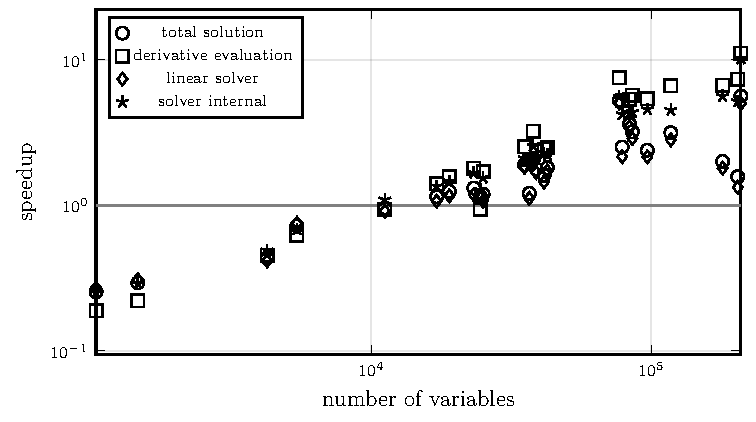
\includegraphics[width=.45\textwidth]{speedup-sol.pdf}
  \caption{Speedup achieved by using GPUs.}
  \label{fig:speedup}
\end{figure}

\paragraph*{Convergence pattern}
First, when comparing the solvers' performance in terms of the
interior point method (IPM) iteration counts, MadNLP.jl is as
efficient as the state-of-the-art solver Ipopt. The IPM iteration
count is nearly the same as that of Ipopt for achieving the same level
of accuracy in the final solution (see Table \ref{tbl:quality}). This
suggests that running mathematically equivalent operations on GPUs (by
using shared code base in high-level abstractions) can yield a similar
degree of effectiveness in terms of IPM convergence.

\paragraph*{Performance of AD}
Next, we discuss the effectiveness of parallel AD on GPUs. We observe
that even on CPUs, SIMDiff.jl is substantially faster than the AD
routines implemented in AMPL or JuMP.jl. Indeed, SIMDiff.jl generates
derivative functions specifically compiled for the type of model,
including optimization for the distinctive computational pattern found
in the model. When comparing SIMDiff.jl running on CPUs and GPUs, we
observe a further speedup on the GPU of up to almost 20x for large
instances (e.g., case24465\_goc); remarkably, this is 500 times faster
than JuMP.jl. This demonstrates that adopting SIMD abstraction and
parallelizing AD brings significant computational gain. 

\paragraph*{Performance of the Condensed-Space IPM}
We next discuss the linear solver time. While the speedup achieved by
linear solvers is only moderate, this has a high impact on the overall
speedup, as linear solver time constitutes a significant portion of
the total solution time. For large instances, approximately 4x speedup
can be achieved, though this can vary depending on the instances. For
example, for case24464\_goc, the GPU linear solver was slower than the
CPUs. The investigation of under which circumstances {\tt cuSOLVERRF} is
more effective warrants further research.

Solver internal time could also be significantly accelerated through
GPU utilization. We can observe that the speedup in solver internal
operations is consistently greater than the speedup in linear
solvers. However, due to the frequent use of \ref{eqn:pattern-2} and
\ref{eqn:pattern-3} operations, the speedup in solver internal
operations is lesser than that of derivative evaluations.

Overall, our GPU implementation exhibits significant speedup across
all components (derivative evaluation, linear algebra, and solver
internal computation) resulting in substantial gains in total solution
time. The results indicate that GPUs become more effective for
large-scale instances, particularly when the number of variables is
greater than 20,000. Notably, for the largest instance,
case30000\_goc, our GPU implementation is 4 times faster than our CPU
implementation and approximately 10 times faster than
state-of-the-art tools (Ipopt, JuMP.jl, and Ma27).
This demonstrates that GPUs can bring significant computational
gains for large-scale AC OPF problems, enabling the solution of
previously inconceivable problems due to the limitations of CPU-based
solution tools.

\paragraph*{Known Limiataions}
The key limitation of our method is the decreased precision of the
final solution. Reliable convergence is achieved only up to a
tolerance of $10^{-4}$. We have observed that the condensation of the
KKT system worsens the conditioning of the already ill-conditioned
augmented KKT system, resulting in even higher condition numbers,
particularly when the solution is almost converged. For instance, in
the case of case118\_ieee, the condition number of the KKT system at
the solution (with tolerance set to $10^{-4}$) is $9.43\times 10^{11}$
for the augmented KKT system and $3.15\times 10^{14}$ for the
condensed KKT system. As a consequence, the achievable precision of
the solution is reduced. Further investigation into the possibility of
obtaining higher precision will be necessary in the future.

\section{Conclusions and Future Outlook}\label{sec:conc}
We have presented an NLP solution framework for solving large-scale AC
OPF problems. By leveraging the SIMD abstraction of NLPs and a
condensed-space IPM, we have effectively eliminated the need for
serial computations, enabling the implementation of a solution
framework that can run entirely on GPUs. Our method has demonstrated
promising results, achieving a 4x speedup when compared to CPU
implementations for large-scale AC OPF problems. Notably, our approach
outperforms one of the state-of-the-art CPU-based implementations by
a factor of 10. These results, along with our packages
MadNLP.jl and SIMDiff.jl, showcase a significant advancement in our
capabilities in dealing with large-scale optimization problems in
power systems and underscore the potential of accelerated computing in
large-scale optimization area. However, the condensation procedure
leads to an increase in the condition number of the KKT system,
resulting in decreased final solution accuracy. Addressing the
challenges posed by ill-conditioning remains to be an important aspect
for future work. In the following paragraphs, we discuss some
remaining open questions and future outlooks.

\paragraph*{Obtaining Higher Numerical Precision}
While we have focused on the IPM, other constrained optimization
paradigms, such as penalty methods and augmented Lagrangian methods
exist, and similar strategies based on condensed linear systems can be
developed. It would be valuable to investigate which algorithm would
be the right paradigm for constrained large-scale optimization on GPU
that can best handle the ill-conditioning issue of the condensed KKT
system, and in turn, achieve the highest degree of accuracy.

\paragraph*{Security-Constrained, Multi-Period, Distribution OPFs}
Though the proposed method has demonstrated significant computational
advantages for transmission AC OPF problems, our results can also
interpreted that efficient CPUs can still handle these problems
reasonably well. We anticipate that there will be more substantial
performance gains for larger-scale optimization problems, such as
security-constrained and multi-period OPFs or joint optimization
problems involving transmission, distribution, and gas network
systems. We are interested in exploring Schur complement-based
decomposition approaches, combined with the condensation-based
strategy, similarly to \cite{pacaud2023parallel}, to demonstrate even
greater scalability.

\paragraph*{Alternative Linear Solvers}
While {\tt cuSOLVERRF} has been effective for solving the condensed KKT
systems using LU factorization, Cholesky factorization holds promise
for better performance due to lower computational complexity and the
ability to reveal the inertia of the KKT system. In the future, we are
interested in exploring other linear solvers options, such as CHOLMOD
\cite{chen2008algorithm}, Baspacho \cite{pineda2022theseus}, and HyKKT
\cite{regev2023hykkt}.

\paragraph*{Portability}
Our implementation is currently only tested on NVIDIA GPUs, but our
GPU implementation is largely based on array programming and
KernelAbstractions.jl in Julia, which are in principle  compatible with
various GPU architectures, including AMD, Intel, and Apple GPUs. By
incorporating cross-architecture linear solvers, we envision
supporting broader class of GPU accelerators in the future.


\bibliographystyle{ieeetr}
\bibliography{main}
\vspace{0.1cm}
\begin{flushright}
  \scriptsize \framebox{\parbox{2.5in}{Government License: The
      submitted manuscript has been created by UChicago Argonne,
      LLC, Operator of Argonne National Laboratory (``Argonne").
      Argonne, a U.S. Department of Energy Office of Science
      laboratory, is operated under Contract
      No. DE-AC02-06CH11357.  The U.S. Government retains for
      itself, and others acting on its behalf, a paid-up
      nonexclusive, irrevocable worldwide license in said
      article to reproduce, prepare derivative works, distribute
      copies to the public, and perform publicly and display
      publicly, by or on behalf of the Government. The Department of Energy will provide public access to these results of federally sponsored research in accordance with the DOE Public Access Plan. http://energy.gov/downloads/doe-public-access-plan. }}
  \normalsize
\end{flushright}

\end{document}


